\section{Experiment}
We say the problem is two-spiral classification. First, we plot the training set contained 96 examples on Figure 1.

\begin{figure}
\centering
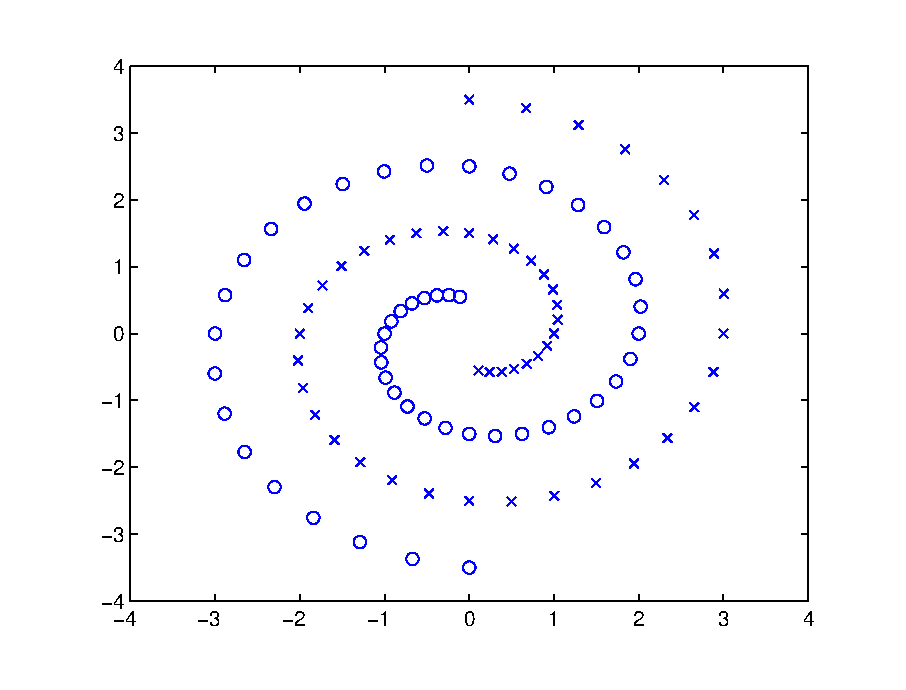
\epsfig{file=trainExamples.eps,width=0.9\columnwidth}
\caption{Training set examples plotting}
\end{figure}

The batch learning MLQPs model achieves 100 \% on both training set and testing set examples. The figure 2 shows the experiment result. Figure 3 illustrates the tends that cost function changed with iterations.

\begin{figure}
\centering
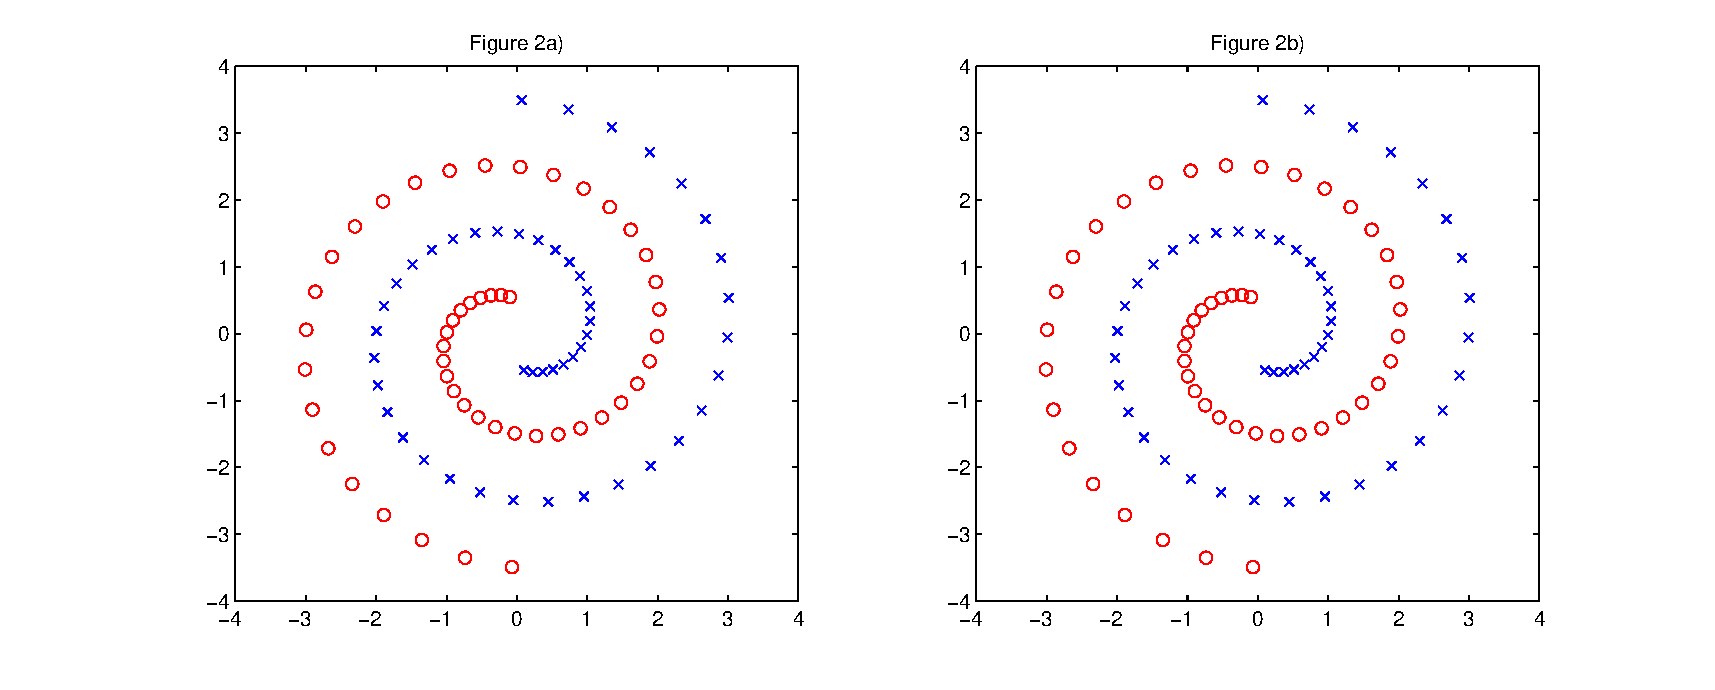
\epsfig{file=batchCompare.eps,width=\columnwidth}
\caption{Batch learning result on test set. Figure 2a) plot the test set examples; Figure 2b) plot the prediction result on the test set examples using batch learning MLQPs model}
\end{figure}

The precision of the result on test set examples using batch learning MLQPs model is 100 \%. We can see that Figure 2a) and Figure 2b) exactly match well on each other.

Figure 3 separately illustrates two different classification regions of MLQPs model for this training data set in red color and blue color.
\begin{figure}
\centering
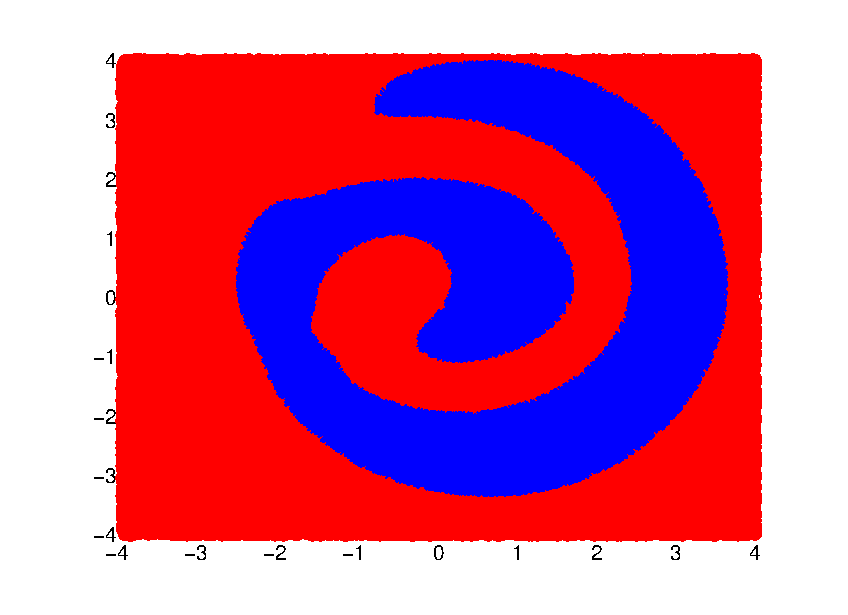
\epsfig{file = decision.eps,width=0.9\columnwidth}
\caption{Decision Region, the red region and blue region represents for two different classes region in the problem. }
\end{figure}

We also do the experiment to compare the two algorithms (batch algorithm and online algorithm) for running time. Using the simple gradient descent optimization algorithm, the batch learning algorithm costs 19.227 seconds, while the online learning algorithm costs about 5.522 seconds. Both of the batch learning algorithm and the online learning algorithm have 100 \% precision. However, batch algorithm speeds up to 2.695 seconds after adopting the \textbf{advanced optimization} algorithm L-BFGS.

